\chapter{Analiza tematu wyszukiwania tekstu}  % Analiza tematu
% 

%\begin{itemize}
%\item Jaki problem chcę (muszę :-) rozwiązać?
%\item Dlaczego rozwiązanie problemu jest ważne?
%\item Jak inni rozwiązują ten problem?
%\item Jakie są zalety i wady tych rozwiązań?
%\end{itemize}

%Odwołania do literatury:
%książek \cite{bib:ksiazka},
%artykułów w czasopismach \cite{bib:artykul},
%materiałów konferencyjnych \cite{bib:konferencja}
%i stron www \cite{bib:internet}.
%
%Równania powinny być numerowane
\begin{align}
    y = \frac{\partial x}{\partial t}
\end{align}
%
%
%\begin{itemize}
%\item analiza tematu
%\item wprowadzenie do dziedziny (\english{state of the art}) – sformułowanie problemu, 
%\item poszerzone studia literaturowe, przegląd literatury tematu (należy wskazać źródła wszystkich informacji zawartych w pracy)
%\item opis znanych rozwiązań, algorytmów, osadzenie pracy w kontekście
%\item Tytuł rozdziału jest często zbliżony do tematu pracy. 
%\item Rozdział jest wysycony cytowaniami do literatury \cite{bib:artykul,bib:ksiazka,bib:konferencja}. 
%Cytowanie książki \cite{bib:ksiazka}, artykułu w czasopiśmie \cite{bib:artykul}, artykułu konferencyjnego \cite{bib:konferencja} lub strony internetowej \cite{bib:internet}.
%\end{itemize}

\begin{Definition}\label{def:1}
Definicja to zdanie (lub układ zdań) odpowiadające na pytanie o strukturze „co to jest a?”. Definicja normalna jest zdaniem złożonym z 2 członów: definiowanego (łac. definiendum) i definiującego (łac. definiens), połączonych spójnikiem definicyjnym („jest to”, „to tyle, co” itp.). 
\end{Definition}

\begin{Theorem}[Pitagorasa]\label{t:pitagoras}
W dowolnym trójkącie prostokątnym suma kwadratów długości przyprostokątnych jest równa kwadratowi długości przeciwprostokątnej tego trójkąta. 
\end{Theorem}

\begin{Example}[generalizacja]\label{ex:generalizacja}
Przykładem generalizacji jest para: zwierzę i pies. Pies jest zwierzęciem. Pies jest uszczegółowieniem pojęcia zwierzę. Zwierzę jest uogólnieniem pojęcia pies.
\end{Example}
\section{Sformułowanie problemu}
Wyszukiwanie tekstu w systemach towarzszy ludziom od początków istnienia maszyn,
choć pierwsze komputery nie posiadały ogromnych ilość pamięci co nie powodowało
potrzeby istnienia algorytmów wyszukujących tekst. Procesor Intel 8008 
zaprezentowany w 1972 posiadał jedynie 14 bitową magistrale adresową co 
pozwalało na 16 Kbi pamięci. Model Motoroli 68000 posiada 5 MB dysku twardego,
co nie może się równać z opecnym standardem darmowej pamięci udostępnianej w 
chmurze przez Google (15 GB).

Zasadniczym problem naszej pracy jest wyszukiwanie zawartości tekstowej
ogramnej ilość plików w różnych formatach. Takie podejście może okazać się 
problematyczne w przypadku plików dzwiękowych, filomowych czy zdjęć wszelkiego
rodzaju.

\section{State of art}

Podjęcie problemu wyszukiwania plików po nazwach oraz zawartości jest bardzo
złożonym i trudnym problemem w sferze programistycznej. Istnieje wiele rozwiązań
tego problemu, które istnieją od początku pracy z komputerem. Narzędzia takie
jak \textbf{find}, \textbf{grep} czy \textbf{fzf} \cite{bib:internet:Fzf} pozwalają na wyszukiwanie
zawartości która nas interesuje, ale kompleksowość tych narzędzi nie jest 
przystosowana do tak trudnego problemu, jakim jest wyszukiwanie treści w plikach,
które są zarchiwizowane. Z taką samą niedogodnością spotykamy się w przypadku
plików pochodzących z pakietu Microsoft Office 365, jednak jeśli rozwiążemy 
zadanie otrzymywania zawartości z archiwów, będziemy w stanie otrzymać również 
zawartość z plików z rozszerzeniami .doc, .docx czy .pptx.

\subsection{Przykładowe narzędzia dostępne do wykorzystania}

Narzędzie \textbf{find} to znane i popularne narzędzie wśród osób zaznajomionych z
technologiami linuxowymi. Już bardzo często wykorzystywany do znajdowania plików
w systemie, jednak nie nadaje sie do znajdowania zawartości plików.

Przykłady użycia programu find:
\begin{itemize} 
  \label{fig:find-example}
  \item find rootPath -name '*.ext'
  \item find rootPath -path 'path/*.ext' 
  \item find rootPath -name '*.py' -not -path '*/site-packages/*'
  \item find rootPath -maxdepth 1 -size +500k -size -10M
  \item find rootPath -type f -empty -delete
\end{itemize}
%\begin{figure}[h]
%  \centering
%  \begin{lstlisting}
%  \end{lstlisting}
%  \caption{Przykłady użycia programu find}
%  \label{fig:code:bashFindExamples}
%\end{figure}

Do przeszukiwania zawartości plików dobrze nadaje się narzędzie grep, który jest
dostępny w każdej dystrybucji Linuxa. Jego działanie jest dość podobne do finda,
lecz posiada on możliwość wyszukiwania treść w plikach tekstowych, lecz nie w 
archiwach. Grep nie posiada też możliwość szukania zawartości plików .pdf oraz
nie wspiera formatów książkowych takich jak .djvu.

Przykłady użycia programu find:
\begin{itemize} 
  \label{fig:grep-example}
  \item grep "searchPattern" path/to/file
  \item grep -F|--fixed-strings "exactString" path/to/file
  \item cat path/to/file | grep -v|--invert-match "searchPattern"
\end{itemize}

Istnieje również ripgrep, który jest sukcesorem wcześniej wymienionego
narzędzia. Jego wydajność przewyższa grepa nawet trzydziestokrotnie w niektórych
testach sprawnościowych, jednak zazwyczaj jest to niewielki wzrost. Nie jest on
niestety domyślnie instalowany na większości systemów linuxowych. Nie posiada on
również wsparcia dla formatów pdf i djvu.

Można wyszukiwać również po treści piosenek, ale wymagałoby to utworzenie modelu
sztucznej inteligencji, która wydobywałaby tekst z piosenek do postaci tekstowej.

\section{Odniesienia do literatury}

Istnieje wiele odniesień do wyszukiwania danych w literaturze. Praca Google 
\cite{bib:internet:htmlSearchGoogle} odnosi się do problemu wyszukiwania tekstu 
w dobie internetu i ilości danych, która jest przechowywana w chmurze. Wymagane
jest indeksowanie, które przyspiesza wyszukiwanie, ale wykonane nie poprawnie 
skutkuje słabymi wyszukiwaniami. Ilość danych wydobywana i dostarczana do
użytkowników stanowi duże wyzwanie oraz wymaga wykorzystania skomplikowanych 
algorytmów. 

Należy również mieć świadomość, że wyszukiwanie tekstu html posiada dodatkową 
złożoność związaną z linkami (ang. \english{anchor}). Linki mogą prowadzić do 
kolejnych stron lub plików, które należy przeszukać w celu wydobycia informacji.
Powoduje to, że proste wyszukiwanie wymaga adaptacji kodu, aby odnieść się do 
przypadków o których wcześniej nie wiedziano.

W plikach, które znajdują się na stronach mogą być na przykład archiwa, które
mają różne wielkości oraz różne typy kompresji. Dodatkowo kompresja może być 
bardziej agresywna lub nawet stratna.

Podczas konferencji TREC \cite{bib:konferencja:TRECDuplicates} jeden z zespołów 
napotkał problem, duplikacji danych. Chęć wydobycia danych w celu utworzenia
tekstów wymagało odpowiedniej deduplikacji dokumentów oraz wyborze tej treści,
która posiada najwięcej wartości. Mogłoby to być tematem rozszerzenie pracy. 

\textbf{TODO MORE PAPERS ADDED}

\section{Opis poznanych rozwiązań}
\subsection{Algorytm brute force}

Jest wiele algorytmów, które wyszukują tekst. Jednym z takich algorytmów jest 
algorytm typu brute-force. Polega sprawdzaniu każdego bajtu, jego implementacja
jest bardzo prosta i standardowa, a złożoność czasowe tego rozwiązania wynosi
O(m * n), gdzie m to długość bloku (pattern), a n to długość tekstu (substring) 
wyszukiwanego. Ten sposób odnajdywania sprawdza się jednak tylko w przypadku,
gdy pattern jest niezbyt długi. Przykładową implementacje algorytmu można 
znaleźć na rysunku \ref{fig:code:bruteForceComparison}.

\begin{figure}[h]
  \centering
  \begin{lstlisting}
for i := 0; i<len(pattern); i++{
  for j := 0; j<len(substring); j++{
    // compare bytes
  }
}
  \end{lstlisting}
  \caption{Przykłady algorytmu brute force}
  \label{fig:code:bruteForceComparison}
\end{figure}

Zaletą tego algorytmu jest to, że nie posiada potrzeby przechowywać żadnych 
danych w pamięci. Ten algorytm dobrze sprawdza się, gdy posiadamy ograniczoną 
ilość zasobów pamięci, co nie jest problemem w obecnych czasach, gdy pamięć jest
stosunkowo tania i szeroko dostępna \ref{screenshot:MemPrices}.
\begin{figure}[h]
  \centering
  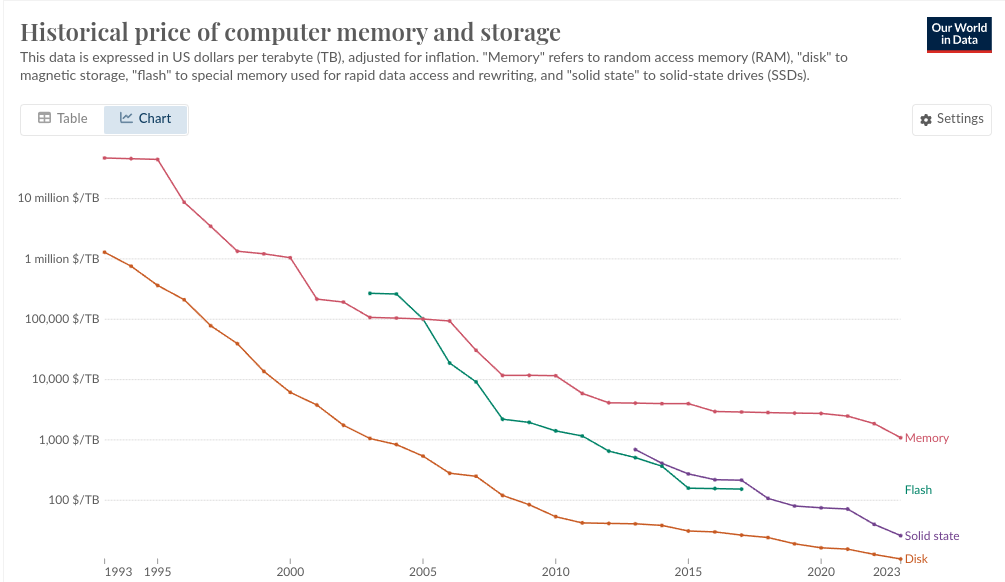
\includegraphics[width=0.9\textwidth]{./images/historical-mem-price.png}
  \caption{Historyczne dane cen pamięci w latach 1993-2023 }
  \label{screenshot:MemPrices}
\end{figure}
%\cite{internet:HistoricalMemPrice}
%https://jcmit.net/memoryprice.htm

Powyższy algorytm można zrównoleglić, dzieląc wzorzec na mniejsze części
i wyszukując tylko dane w tym obszarze \ref{tabela:NormalProblemBruteForce}, 
ale należy dołożyć końce wzorca, aby nie wynikła sytuacja, w której wzorzec by
wystąpił, ale nie wzięto pod uwagę końca zdania. 

\begin{table}
  \centering
  \begin{tabular}{ |c|c|  } 
    \hline
    \multicolumn{2}{|c|}{Metoda Brute Force} \\
    \hline
    wzorzec & ABCABCABDABD \\
    \hline
    podłańcuch & BCA \\
    \hline
    rezultat & 4 \\
    \hline
  \end{tabular}
  \caption{Zwykły problem wyszukiwania metodą brute force}
  \label{tabela:NormalProblemBruteForce}
\end{table}


\begin{table}
  \centering
  \begin{tabular}{ |c|c||c|c|  } 
    \hline
    \multicolumn{4}{|c|}{Zadania} \\
    \hline
    Zadanie 1 & & Zadanie 2 & \\
    \hline
    wzorzec & ABCABC & wzorzec & ABDABD \\
    \hline
    podłańcuch & BCA & podłańcuch & BCA \\
    \hline
    rezultat & -1 & rezultat & -1 \\ 
    \hline
  \end{tabular}
  \caption{Zwykły problem wyszukiwania metodą brute force}
  \label{tabela:splitTasksBruteForce}
\end{table}

Jeżeli podzielimy wzorzec na dwa procesy wyszukujące algorytmem brute-force,
otrzymamy dwa zadania \ref{tabela:splitTasksBruteForce}. Zrównoleglenie procesu 
powoduje, że otrzymaliśmy nie poprawny wynik, gdyż w żadnym z wzorców nie
występuje podłańcuch "BCA", choć łańcuch występuje w miejscu 4, to algorytm nie
posiada wiedzy o dalszej części wzorca.

\begin{table}
  \centering
  \begin{tabular}{ |c|c||c|c|  } 
    \hline
    \multicolumn{4}{|c|}{Zadania} \\
    \hline
    Zadanie 1 & & Zadanie 2 & \\
    \hline
    wzorzec & ABCABC(AB) & wzorzec & ABDABD(nil) \\
    \hline
    podłańcuch & BCA & podłańcuch & BCA \\
    \hline
    rezultat & 4 & rezultat & -1 \\ 
    \hline
  \end{tabular}
  \caption{Zwykły problem wyszukiwania metodą brute force}
  \label{tabela:splitBruteForceCorrected}
\end{table}

Aby poprawić dany algorytm należy dołożyć znaki, które należy sprawdzać w 
przypadku poprawnego rozpatrzenia ostatniego znaku 
\ref{tabela:splitBruteForceCorrected}. W takim przypadku sprawdzamy tylko do
sytuacji, w której BC jest częścią podłańcucha, ale podłańcuch nie został w 
pełni znaleziony. Długość ponownego wyszukania byłaby równa len(podłańcuch) - 1.


\subsection{Algorytm Morisa-Pratta}

Algorytm Morisa-Pratta jest dość prostym algorytmem wykorzystującym możliwość
wcześniejszego sprocesowania podłańcucha wyszukiwanego w tekście co przyspiesza
sposób procesowania tekstu jak na rysunku \ref{fig:code:preprocessMorisPratt}.
Polega on na wykorzystaniu faktu istnienia pasującego prefikso sufiksu.
Pozwala to na pominięcie pewnych porównania niektórych znaków, bez szkody w
wyniku wyszukiwania.

Dzięki wykorzystaniu tej zależności możemy uniknąć cofania się indeksu i. 
Tablice preproc wypełniamy poprzednią wartości tak długo, aż zaistnieje różnica 
pomiędzy obecnym a następnym znakiem tablicy substr. W przypadku różnicy 
zwiększamy wartość zapisywaną do tablicy preprocesora o odległość różnicy znaków.
W ten sposób następnym razem będzie możliwość pominięcia porównania tych znaków.

\begin{figure}[h]
  \centering
  \begin{lstlisting}
curr = -1
preproc[0] = -1
for i := 1; i <= len(substr); i++ {
  for (curr > -1) && (substr[curr] != substr[i-1]) {
    curr = preproc[curr]
  }
  curr++
  preproc[i] = curr
}
  \end{lstlisting}
  \caption{Przykład preprocesowania podłańcucha}
  \label{fig:code:preprocessMorisPratt}
\end{figure}

W drugim etapie można wykorzystać wcześniej przygotowaną tablice przemieszczeń 
\textbf{preproc}, aby obliczyć ilość przesunięcia w przypadku znalezienia 
niepasującego prefiksu \ref{fig:code:algoMorisPratt}. Dzięki temu zwykle dłuższy tekst znajdujący się w 
\textbf{wzorcu s} możemy przeanalizować szybciej, niż w przypadku algorytmu 
bruteforce. Powoduje to niestety problem w przypadku, gdy wyszukiwany wzorzec
nie jest wystarczająco długi, gdyż wykonanie operacji preprocesu posiada 
dodatkowy koszt, którego nie ma w algorytmie brute force.

\begin{figure}[h]
  \centering
  \begin{lstlisting}
res := []int{}
curr := 0
found := 0
for i := 0; i < len(s); i++ {
  for (curr > -1) && (substr[curr] != s[i]) {
    curr = preproc[curr]
  }
  curr++
  if curr == len(substr) {
    for found < i-curr+1 {
      found++
    }
    res = append(res, found)
    found++
    curr = preproc[curr]
  }
}
  \end{lstlisting}
  \caption{Przykład preprocesowania podłańcucha }
  \label{fig:code:algoMorisPratt}
\end{figure}

\begin{figure}[h]
  \centering
  \begin{lstlisting}
func Index(s, substr string) int {
  n := len(substr)
	switch {
	case n == 0:
		return 0
  [...]
	case n > len(s):
		return -1
	case n <= bytealg.MaxLen: // Usually this case is used
		// Use brute force when s and substr both are small
		if len(s) <= bytealg.MaxBruteForce /* max == 64 */{
			return bytealg.IndexString(s, substr)
		}
  [...]
  }
}
  \end{lstlisting}
  \caption{ Szukanie łańcucha w standardowej bibliotece Golang }
  \label{fig:code:golangSearchInsideString}
\end{figure}

W podstawowej bibliotece języka Golang, w pakiecie \textit{strings} istnieje 
implementacja metody \textit{Index()}. Nie jest ona jednak w pełni przedstawiona
w kodzie, natomiast w jej implementacji można zauważyć, że algorytm brute force
jest wykorzystywany tylko w przypadku, gdy długość wzorca wynosi więcej niż 64 
\ref{fig:code:golangSearchInsideString}. W Golang, gdy wzorzec jest większy niż
64 znaki, to wykonuje się algorytm podobny do Morisa-Pratta, który jednak 
posiada dodatkową walidacje w przypadku odkrycia false positives. 
Algorytm Morisa-Pratta nie potrzebuje takiej walidacji.


\subsection{Algorytm Kurta-Morisa-Pratta}

\begin{listing}[H]
    \begin{minted}[xleftmargin=0.15\textwidth,xrightmargin=0.2\textwidth,linenos]{diff}
preproc := make([]int, lensubstr+1)
preproc[0] = -1
curr := -1
for i := 1; i <= lensubstr; i++ {
  for (curr > -1) && (substr[curr] != substr[i-1]) {
    curr = preproc[curr]
  }
  curr++
- preproc[i] = curr
+ if (i == lensubstr) || (substr[i] != substr[curr]) {
+   preproc[i] = curr
+ } else {
+   preproc[i] = preproc[curr]
+ }
}
mp.preproc = preproc
    \end{minted}
  \caption{Różnica pomiędzy algorytmami KMP i MP}
  \label{fig:code:KurtMorisPrattVsMorisPratt}
\end{listing}

Kolejnym algorytmem, który rozpatrujemy jest implementacja rozszerzająca 
poprzednią implementacje. Różnice można zauważyć na podstawie rysunku
\ref{fig:code:KurtMorisPrattVsMorisPratt} i polega ona na dodatkowym sprawdzeniu
gdy nie osiągnieliśmy długości łańcucha i obecny znak jest równy temu, który 
znajduje się w podłańcuchu to możemy wykonać skok do elementu znajdującego
sie w tablicy przygotowanej, a nie zostawać w obecnym puncie pętli. Ta różnica
powoduje, że algorytm wykonuje się szybciej.

Złożoność tego algorytmu wynosi $O(2*{k})$ co mieści się w złożoności $O({k})$,
gdzie k jest długością wzorca, w którym podłańcuch jest wyszukiwany. W 
najbardziej pesymistycznym przypadku, gdy próba dopasowania tekstu będzie 
kończyć się porażką, będzie wymagało to $O({n})$ operacji co nie jest szybsze,
niż algorytm naiwny. 

\begin{table}
  \centering
  \begin{tabular}{ |c|c|  } 
    % \hline
    % \multicolumn{2}{|c|}{Przykład wykorzystania algorytmu KMP} \\
    \hline
    wzorzec S & AAAAAABAAAAAABAAAAAAA \\
    \hline
    podłańcuch W & AAAAAA \\
    \hline
    liczba cofnięć & 20 \\
    \hline
  \end{tabular}
  \caption{Przykład wykorzystania algorytmu KMP}
  \label{tabela:KMPExampleSlow}
\end{table}

Wzorzec T przedstawia najbardziej niekorzystny scenariusz 
\ref{tabela:KMPExampleSlow}, co można zaobserwować na przykładzie tekstu 
S = "AAAAAABAAAAAABAAAAAAA". W tym przypadku algorytm musi sprawdzić każde
wystąpienie 'A' przed dotarciem do 'B', co jest bardzo nieefektywne. Sytuacja 
pogarsza się wraz ze wzrostem liczby powtórzeń fragmentu "AAAAAAB". Mimo że 
metoda tablicowa działa tu sprawnie (bez potrzeby cofania się), to jej 
jednokrotne wykonanie dla podłańcucha W może być wolny, gdyż proces
wyszukiwania często wymaga wielokrotnych przebiegów. Wielokrotne przeszukiwanie
tekstu S w poszukiwaniu wzorca prowadzi do gorszej wydajności. W takich 
przypadkach, gdzie mamy do czynienia z tego typu charakterystyką tekstu 
i wzorca, algorytm Boyera-Moore'a może stanowić optymalne rozwiązanie.

Algorytm KMP wykorzystuje w najgorszym przypadku liniowy przebieg, natomiast
algorytm Boyera-Moore'a w najlepszym przypadku posiada złożoność $O(n+k)$, a w 
najgorszym przypadku $O(n*k)$, gdzie n jest długością podłańcucha.

\subsection{Algorytm Boyera-Moore'a}
\label{sch:algoBoyerMoore}

Zaletą algorytmu jest to, że ilość skoków pomiędzy porównaniami jest zwykle 
większa od 1, a gdy istnieje sytuacja, w której litery w podłańcuchu nie
potwarzają się, to możemy przeskoczyć o długość całego łańcucha.

Algorytm Boyera-Moore'a wprowadza rewolucyjne podejście poprzez skanowanie 
wzorca od prawej do lewej strony, w przeciwieństwie do MP i KMP, które 
analizują tekst od lewej do prawej. Ta fundamentalna różnica pozwala BM na 
znacznie efektywniejsze przeskakiwanie fragmentów tekstu, które na pewno nie 
zawierają wzorca. BM wykorzystuje dwie heurystyki: "złego znaku" oraz "dobrego
sufiksu", podczas gdy KMP i MP opierają się na pojedynczej tablicy prefiksowej.

W kontekście implementacji, BM wymaga utworzenia dwóch tablic pomocniczych dla
swoich heurystyk, co zwiększa złożoność pamięciową w porównaniu do pojedynczej 
tablicy prefiksowej w KMP i MP. Jednak ta dodatkowa pamięć przekłada się na 
możliwość wykonywania większych skoków w tekście. KMP i MP różnią się między 
sobą głównie w sposobie konstrukcji tablicy prefiksowej - KMP wykorzystuje 
bardziej zaawansowaną technikę, która pozwala na uniknięcie niektórych 
niepotrzebnych porównań występujących w MP.

Praktyczny wybór między tymi algorytmami zależy od charakterystyki danych
wejściowych. BM sprawdza się najlepiej w przypadku długich wzorców i tekstów
napisanych w językach naturalnych, gdzie występuje duża różnorodność znaków.
KMP i MP są bardziej przewidywalne w działaniu i mogą być lepszym wyborem dla 
krótkich wzorców lub tekstów o ograniczonym alfabecie, jak na przykład sekwencje
DNA.

Z tego też powodu należy wykonać heurystykę danych, które są analizowane.
Można to zrobić na kilka sposobów, jednak z powodu iż nie jest to główny temat
pracy zostaną użyte narzędzia potrzebne do takiej analizy.


\subsection{TODO? Algorytm Karpa-Rabina}
\subsection{TODO? Algorytm Aho-Corasick}